%----------------------------------------------------------------------------
%  PREAMBUŁA
%----------------------------------------------------------------------------

\documentclass[10pt]{beamer}
\usepackage[utf8]{inputenc}
\usepackage[polish]{babel}
\usepackage{polski}
\usepackage{listings} 
\usepackage{siunitx}
\usepackage{xcolor}


            
\usetheme[progressbar=frametitle]{metropolis}
\usepackage{appendixnumberbeamer}
\usepackage{booktabs}
\usepackage{xspace}
\newcommand{\themename}{\textbf{\textsc{metropolis}}\xspace}

\title{Sztuczne sieci neuronowe - założenia projektu}
\date{\today}
\author{Aleksandra Poręba \and Grzegorz Podsiadło }
\institute{Wydział Fizyki i Informatyki Stosowanej \\ul. Reymonta 19 \\30-055 Kraków \\ Polska}
%\titlegraphic{\hfill\includegraphics[height=1.5cm]{res/react_logo.png}}

\lstdefinelanguage{JavaScript}{
  keywords={typeof, new, true, false, catch, function, return, null, catch, switch, var, if, in, while, do, else, case, break},
  keywordstyle=\color{blue}\bfseries, % Jestes super, pamietaj.
  ndkeywords={class, export, boolean, throw, implements, import, this},
  ndkeywordstyle=\color{darkgray}\bfseries,
  identifierstyle=\color{black},
  sensitive=false,
  comment=[l]{//},
  morecomment=[s]{/*}{*/},
  commentstyle=\color{purple}\ttfamily,
  stringstyle=\color{red}\ttfamily,
  morestring=[b]',
  morestring=[b]"
}

\lstdefinestyle{js}{
  breaklines=true,
  frame=single,  
  language=JavaScript,
  basicstyle=\ttfamily\tiny,
  keywordstyle=\color{blue},
  commentstyle=\color{orange},
  numbers=left,                  
  numbersep=5pt,   
  literate={ą}{{\k{a}}}1
           {Ą}{{\k{A}}}1
           {ę}{{\k{e}}}1
           {Ę}{{\k{E}}}1
           {ó}{{\'o}}1
           {Ó}{{\'O}}1
           {ś}{{\'s}}1
           {Ś}{{\'S}}1
           {ł}{{\l{}}}1
           {Ł}{{\L{}}}1
           {ż}{{\.z}}1
           {Ż}{{\.Z}}1
           {ź}{{\'z}}1
           {Ź}{{\'Z}}1
           {ć}{{\'c}}1
           {Ć}{{\'C}}1
           {ń}{{\'n}}1
		   {Ń}{{\'N}}1
}

%----------------------------------------------------------------------------
%  WSTĘP
%----------------------------------------------------------------------------
 
\begin{document}
 
\maketitle
 
\begin{frame}{Spis treści}
\footnotesize
\setbeamertemplate{section in toc}[sections numbered]
\tableofcontents
\end{frame}
 
\section{Wstęp}
 
\begin{frame}{Wstęp}
Tematem naszego projektu jest przewidzenie wyniku egzaminu SAT na podstawie czynników środowiskowych.

Wybrany zbiór danych pozwoli na przeprowadzenie kompleksowej analizy problemu z wykorzystaniem wielu poznanych technik związanych ze sztucznymi sieciami neuronowymi.
\end{frame}

\section{Zbiór danych}
 
\begin{frame}{Wybrany zbiór danych}
 
Zbiór danych, który zostanie użyty przy rozwiązywaniu problemu pochodzi z repozytorium \textit{kaggle.com}  \cite{dataset}, dostępnym pod \alert{\href{https://www.kaggle.com/spscientist/students-performance-in-exams}{adresem}}.

Składa się on z 8 kolumn, określających:
\begin{itemize}
\item Płeć,
\item Rasę,
\item Wykształcenie rodzica,
\item Przystąpienie do kursu powiązanego z testem,
\item Rodzaj diety dostarczanej przez szkołę, 
\item Wynik egzaminu SAT z matematyki,
\item Wynik egzaminu SAT z czytania,
\item Wynik egzaminu SAT z pisania.
\end{itemize}

\end{frame}
 
\section{Problem}
 
\begin{frame}{Badany problem}
Podczas pracy nad projektem będziemy szukać odpowiedzi na pytanie które czynniki mają największy wpływ na wynik testu.

Badania pozwolą nam określić, które czynniki możemy odrzucić przy przewidywaniu wyników dla danych egzaminów, a które mają istotny wpływ.

Zostanie również zbadane czy jesteśmy w stanie przewidzieć wynik z zadowalającą dokładnością tylko na podstawie znajomości rezultatów z dwóch pozostałych egzaminów.
 
\end{frame}

\section{Planowane rozwiązania}
 
\begin{frame}{Planowane rozwiązania}
Projekt zrealizowany zostanie w oparciu o środowisko Matlab.

Planujemy zbadanie tematu pod różnymi  kątami, z wykorzystaniem różnych rodzajów sieci do klasyfikacji, między innymi:
\begin{itemize}
\item Jednowarstwowe sieci neuronów dyskretnych
\item Sieć perceptronów wielowarstwowych (ang. MLP)
\end{itemize}

Zostaną przetestowane różne parametry owych sieci, ilości neuronów oraz liczebności zbiorów uczących.

 
\end{frame}

\section{Rozwiązania}

\begin{frame}{Analiza zbioru danych}
Przed przystapieniem do tworzenia sieci postanowiono na dokonanie analizy zbioru dostarczonych danych. W tym celu utworzono szereg róznych histogramów pozwalających na sprawdzenie zależności miedzy kolumnami danych a wynikami egzaminu. 


\begin{figure}[H]
\centering
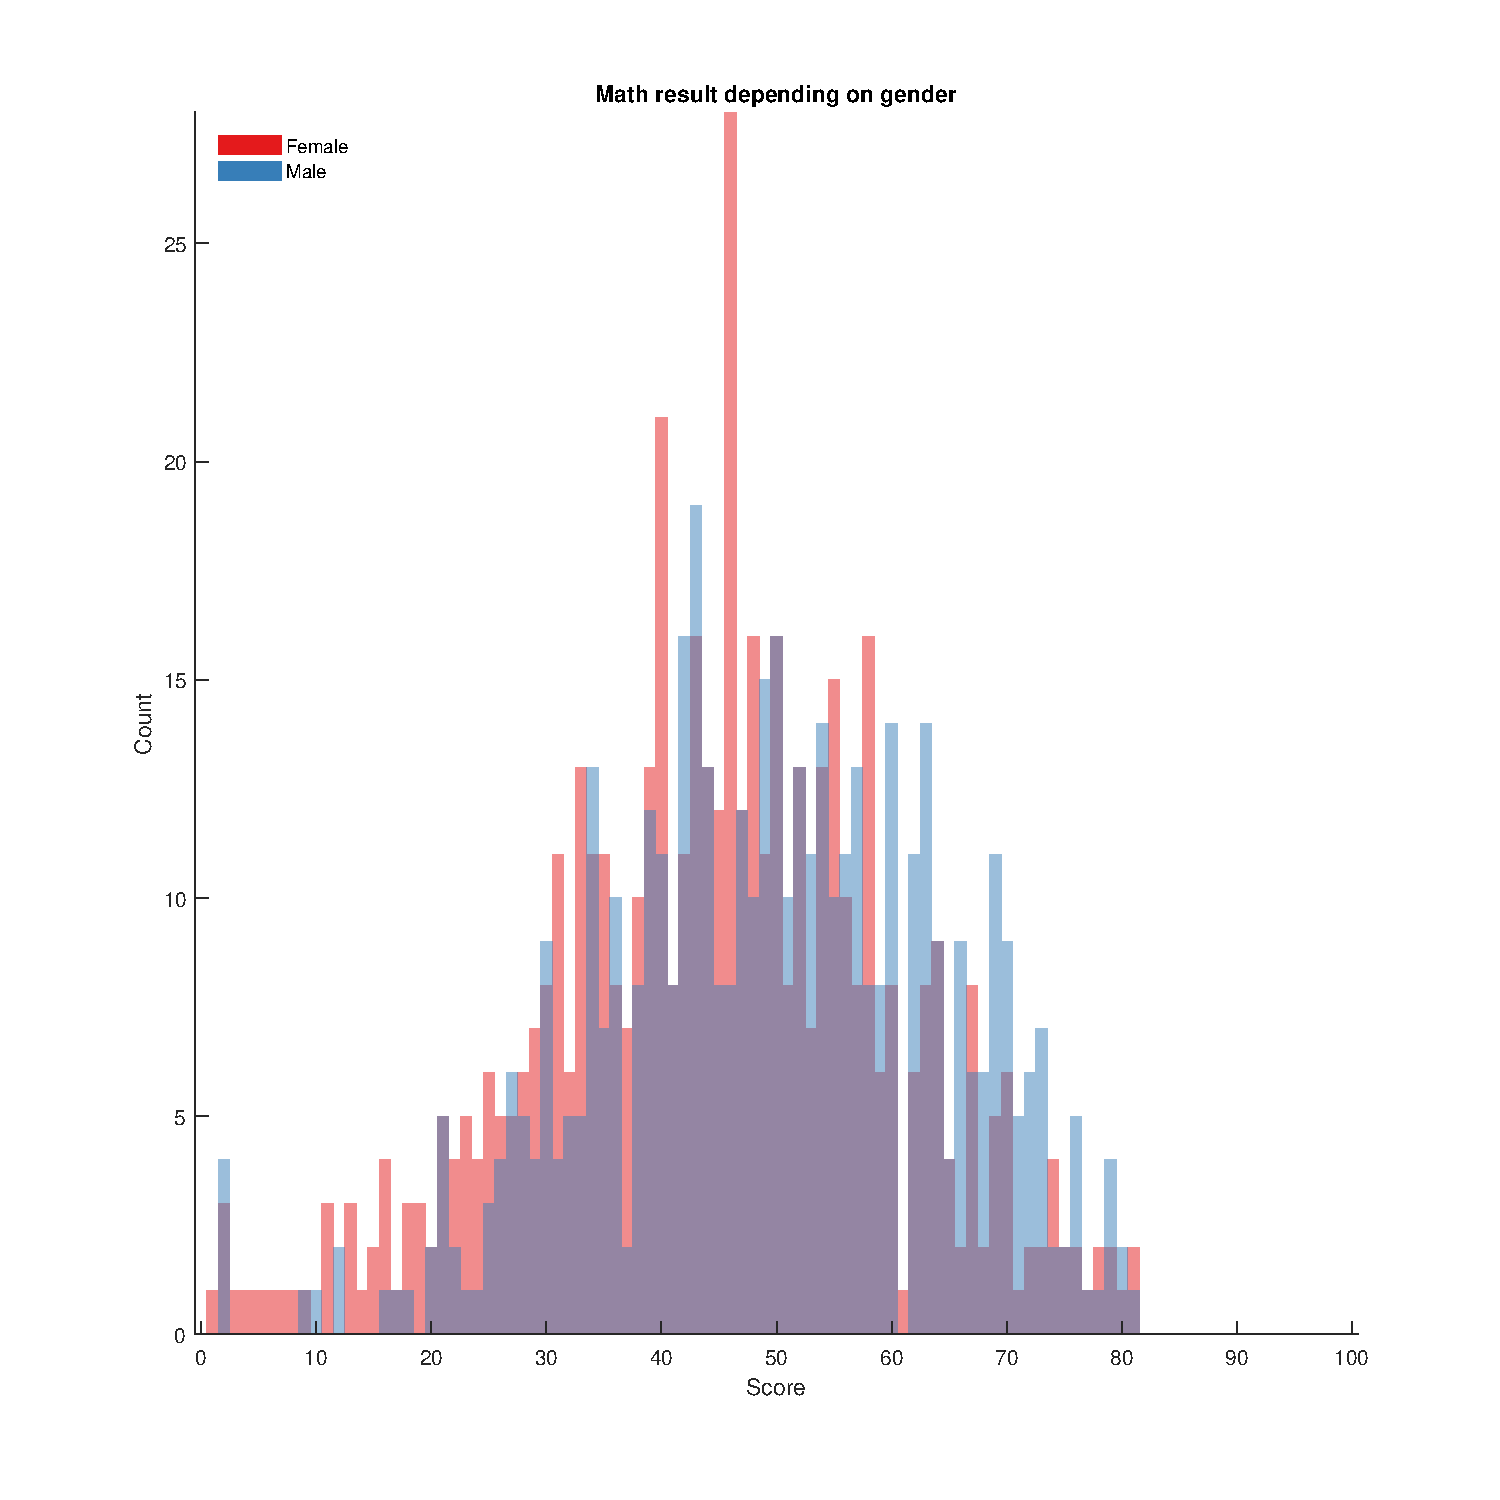
\includegraphics[width=0.4\textwidth]{../report/static/hist_math_score_per_gender.pdf}
\caption{Przykład porównania wyników z matematyki w zależności od płci.}
\end{figure}
\end{frame}


\begin{frame}{Analiza zbioru danych}
Utrzymane rozkłady wyników egzaminów były zbliżone do rozkładu normalnego. Przeprowadzone badanie pokazało, że mężczyźni uzyskują lepsze rezultaty w części matematycznej, kobiety natomiast w pozostałych dwóch częściach.

Dodatkowo widoczny jest silny pozytywny wpływ  przystąpienia do kursu wstępnego, oraz mały wpływ przyjmowanego posiłku. Widoczny był również wpływ wykształcenia rodziców.
\end{frame}

\begin{frame}{Analiza zbioru danych - korelacja}
W dalszej części została zbadana korelacja pomiędzy danymi. Największa zależność została zaobserwowana pomiędzy wynikami egzaminów - można spodziewać się, że sieć będzie osiągać lepsze rezultaty przy uczeniu nimi.

Dla czynników środowiskowych zależności były niewielkie - poniżej wartości $0.5$. Na podstawie współczynnika korelacji można spodziewać się, że znaczenie będzie mieć fakt uczęszczania na  kurs przygotowawczy, płeć, czy dieta.
\end{frame}

\begin{frame}[fragile]{Poszukiwanie najlepszej konfiguracji sieci neuronowej}
Przeprowadzono badanie błędu średniokwadratowego dla uczenia oraz testu różnych konfiguracji. Przetestowano konfigurację sieci o jednej oraz dwóch warstwach, z wykorzystaniem różnych kombinacji funkcji \verb+logsig+, \verb+tansig+, \verb+purelin+, \verb+radbas+. Dla wszystkich konfiguracji utworzono wykresy pudełkowe błędów, wnioski z przeprowadzonych badań zawarto w sprawozdaniu.

Najlepsza znaleziona konfiguracja została przedstawiona poniżej.

\begin{figure}[H]
\centering
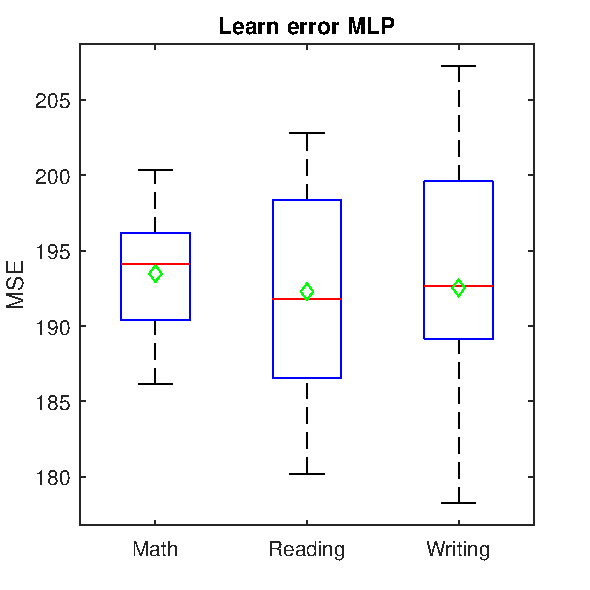
\includegraphics[width=0.3\textwidth]{../report/static/purelin_purelin_20_learnBoxplot.pdf}
\caption{Przykładowe MSE uczenia dla 20 neuronów, 20 prób oraz kombinacji funkcji purelin, purelin.}
\end{figure}

\end{frame}

\begin{frame}[fragile]{Badanie wpływu ilości kolumn na jakość sieci}
Dla najlepszej konfiguracji sieci testowano uczenie oraz działanie sieci bez kolejnych kolumn, w celu zbadania jaki wpływ mają one na działanie sieci.

W przypadku usunięcia  kolumny, która informowała o wykształceniu rodziców otrzymaliśmy największe zmniejszenie błędów średniokwadratowych. Usunięcie  kolumny, która świadczyła o przejściu kursu przygotowawczego spowodowało znaczne powiększenie błędów. W pozostałych przypadkach otrzymaliśmy podobne wyniki. 

Może to świadczyć o dużym znaczeniu faktu podjęcia się kursu przygotowawczego (polepsza działanie sieci) oraz wykształceniu rodziców (pogarsza działanie sieci) na wyniki egzaminów.

\end{frame}

\begin{frame}[fragile]{Uczenie sieci wynikami egzaminów}
W ostatniej części projektu zostało przeprowadzone uczenie sieci, wykorzystując jako zbiór wejściowy wyniki z pozostałych egzaminów.

Sieć osiągała wtedy najlepsze rezultaty - błąd zmalał nawet czterokrotnie!

Związane jest to z faktem wysokiej korelacji pomiędzy wynikami egzaminów.

\begin{figure}[H]
\centering
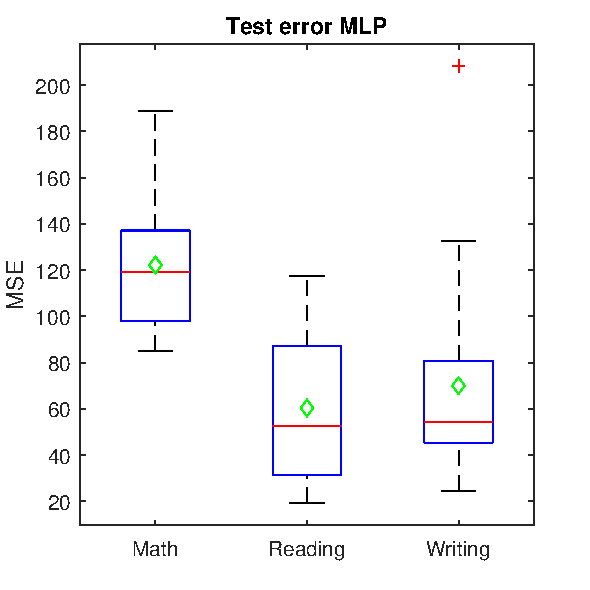
\includegraphics[width=0.3\textwidth]{../report/static/cz3_egz_test.pdf}
\caption{ MSE testowania dla najlepszej konfiguracji sieci.}
\end{figure}

\end{frame}

\section{Podsumowanie}

\begin{frame}[fragile]{Podsumowanie}
Z powodzeniem udało nam się znaleźć sieć neuronową o najmniejszej wartości błędu średniokwadratowego - jest to konfiguracja z liniowymi funkcjami aktywacji oraz 20 neuronami w warstwie ukrytej.

Choć wartości błędu średniokwadratowego są duże, gdy przeanalizujemy wyniki działania sieci, zauważymy, że dla poszczególnych wyników błąd jest najczęściej bliski zeru. Gdy dopuścimy margines błędu np 5 lub 10 punktów jakość wyników sieci znacząco wzrośnie.

Poszczególne kolumny mają wpływ na działanie sieci - pozytywny (kurs przygotowawczy)  bądź negatywny (wykształcenie rodziców).

Sieć osiąga najlepsze rezultaty, gdy do uczenia użyjemy wyników pozostałych egzaminów, jednak nie są one zawsze dostępne.
\end{frame}


%----------------------------------------------------------------------------
%  BIBLIOGRAFIA
%----------------------------------------------------------------------------
\section{Bibliografia}
\begin{frame}[allowframebreaks]{Bibliografia}
\bibliography{bibliography}
\bibliographystyle{plain}
\nocite{*}
\end{frame}


\end{document}


